\documentclass{article}
\usepackage{graphicx}
\usepackage[margin=1.5cm]{geometry}
\usepackage{amsmath}

\begin{document}

\title{Study Guide for Midterm 1: Elementary Statistics}
\author{Prof. Jordan C. Hanson}

\maketitle

\section{Formula Area}

\begin{enumerate}
\item Quantitative continuous data: sample data that can be measured
\item Quantitative discrete data: sample data that can be counted
\item Qualitative or categorical data: sample data that can be classified but not counted
\item Average/mean, definition 1: $\bar{x} = N^{-1} \sum_i x_i$
\item Median: the value below which are half of the frequencies.  Half of the frequencies are also above this value.
\item Mode: the value corresponding to the highest frequendy.
\item The quartiles $Q1$, $Q2$, and $Q3$ are the values that separate the frequencies into four bins of equal frequency. $Q2$ is equal to the median.  The IQR is $Q3 - Q1$.
\item The k-th percentile: the value below which k percent of the data is located.  Formula: $i = (k/100) (n+1)$, where $k$ is the percentile, $n$ is the total number of data, and $i$ is the integer location of the k-th percentile.
\item Finding the percentile of a data value: $(x+0.5*y)/n (100)$, where $x$ is the number of data values below the given data value, $y$ is the number of data values equal to the given one, and $n$ is the total number of data values.
\item Average/mean, definition 2: $\bar{x} = \sum_i^{M} f_{r,i} x_i$, where $x_i$ are the bin centers of a histogram, or the discrete random variable data values, and $f_{r,i}$ are the relative frequencies.  For a discrete random variable, $f_{r,i}$ is replaced with $p(x)$, the probability distribution function.
\item Probabilities of mutually exclusive and independent events: if two events have probabilities $p_1$ and $p_2$, then the probability that event 1 AND event 2 occur is $p_1 p_2$.  The probability that event 1 OR event 2 occurs is $p_1 + p_2$.
\item The standard deviation $s$ of a sample is 
\begin{equation}
s^2 = \frac{1}{N-1}\sum_{i=1} (x-\mu)^2
\end{equation}
\end{enumerate}

\section{Unit 0}

\begin{enumerate}
\item Forbes magazine published data on the best small firms in 2012. These were firms which had been publicly traded for
at least a year, have a stock price of at least \$5 per share, and have reported annual revenue between \$5 million and \$1
billion. Figure \ref{fig:ages} (left) shows the ages of the chief executive officers for the first 60 ranked firms.
\begin{figure}[ht]
\centering
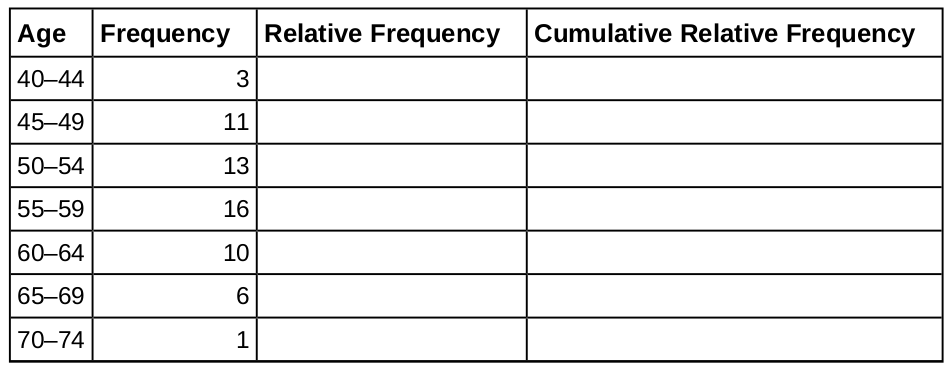
\includegraphics[width=0.45\textwidth]{figures/ages.png}
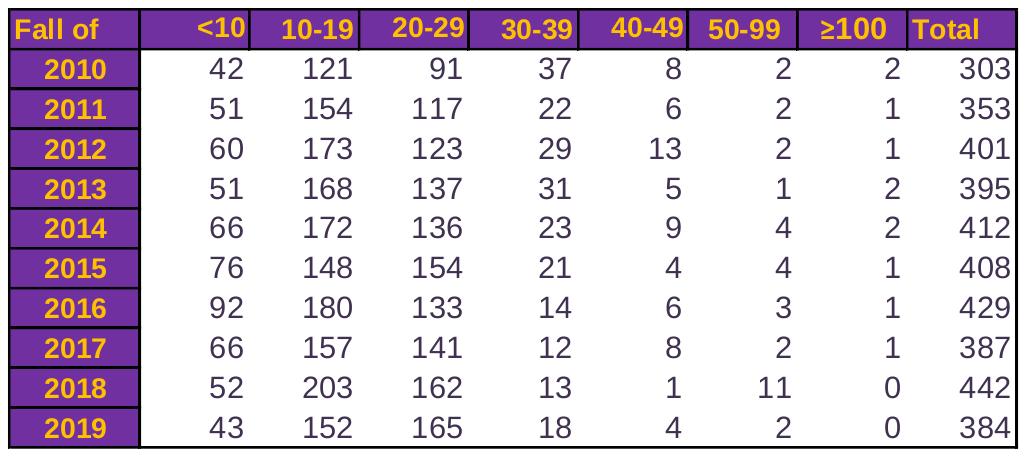
\includegraphics[width=0.4\textwidth]{figures/class_size.png}
\caption{\label{fig:ages} (Left) A table of the ages of CEOs of the top 60 ranked small firms list, according to \textit{Forbes} magazine. (Right) The number of classes at Whittier College, binned by their size, in number of students, and by year. }
\end{figure}
\begin{itemize}
\item What is the frequency for CEO ages between 54 and 65?
\item What percentage of CEOs are 65 years or older?
\item What is the relative frequency of ages under 50?
\item What is the cumulative relative frequency for CEOs younger than 55?
\item Graph the relative the cumulative relative frequency below.
\item Create a Pareto graph of the relative frequencies below.
\end{itemize}
\vspace{2cm}
\item Consider Fig. \ref{fig:ages} (right).
\begin{itemize}
\item Create a time-series plot that contains both the \textit{smallest class size} column, and the \textit{30-39 student} column.  What do you notice? \\ \vspace{2cm}
\item What was the mean class size of Whittier College in 2019? \\ \vspace{1cm}
\item In a particular fund, there are 10 stocks, each with the following price per share in USD: 14,14,15,17,19,21,25,50,72,90.  (a) What is the median?  (b) What price represents the 60th percentile? (c) To what percentile does 19 dollars correspond? (d) What is the standard deviation and mean of the data? \\ \vspace{2cm}
\end{itemize}
\item A lottery is constructed by labeling tokens with all the letters of the alphabet.  There are 26 tokens, and five are drawn, \textit{without replacement.}  If you have to match all five tokens, what are your odds of winning?  (Your card can have any string of five letters, without repeating a letter). \\ \vspace{1cm}
\item Suppose a student is applying to five colleges, each with an equal probability $p$ of accepting him.  (a) What is the probability that he is accepted to all five?  (b) What is the probability that he is accepted to any two of the five colleges? (Think of it like: the first college OR the second college). (c) \textbf{Harder question}: what is the probability he gets accepted to none of them? \\ \vspace{1cm}
\end{enumerate}

\clearpage

\section{Unit 1}

\begin{enumerate}
\item Some stock traders engage in \textit{high frequency trading}, in which they write an algorithm that executes a pre-designed purchase or sale of a stock via computer code that runs for several microseconds.  Suppose the TelCo stock is fluctuating rapidly between \$10 dollars per share and \$20 dollars per share, with an average of \$15 dollars. Consider Tab. \ref{tab:stock} below, which explains the high-frequency strategy.  (a) What is the expectation value of the discrete random variable $x$, the money made per trade? (b) If this code earns the expectation value once per day, after how many days will the profit exceed 100 dollars?  (c) If this code earns the expectation value every 100 microseconds, and runs for 12 hours, what is the profit?
\begin{table}[ht]
\centering
\begin{tabular}{| c | c | c | c |}
\hline
\textbf{Outcome} & $x$ & $p(x)$ & $x*p(x)$ \\ \hline \hline
Buy & -\$14.95 per share & $0.49$ & ? \\ \hline
Sell & +\$15.05 per share & $0.51$ & ? \\ \hline
\hline
\end{tabular}
\caption{\label{tab:stock} The code buys stock when it has a price \$14.95 49, and this occurs 49 percent of the time.  The code sells stock when it has a price of \$15.05, and this occurs 51 percent of the time.} \vspace{2cm}
\end{table}
\item Suppose the trading goes on from the previous problem and the profits for one week days in USD are 1.20, 4.05, 3.45, 0.90, 1.10, 2.40, and 0.50.  What is the standard deviation in the profits?  What is the mean?  How many standard deviations is the last data point \textit{below} the mean?  (That is, how rare is this?).
\end{enumerate}

\end{document}